\chapter{Function operators}\label{function-operators}

In this chapter, you'll learn about function operators (FOs). A function
operator is a function that takes one (or more) functions as input and
returns a function as output. In some ways, function operators are
similar to functionals: there's nothing you can't do without them, but
they can make your code more readable and expressive, and they can help
you write code faster. The main difference is that functionals extract
common patterns of loop use, where function operators extract common
patterns of anonymous function use. \index{function operators}

The following code shows a simple function operator, \texttt{chatty()}.
It wraps a function, making a new function that prints out its first
argument. It's useful because it gives you a window to see how
functionals, like \texttt{vapply()}, work.

\begin{Shaded}
\begin{Highlighting}[]
\NormalTok{chatty <-}\StringTok{ }\NormalTok{function(f) \{}
  \NormalTok{function(x, ...) \{}
    \NormalTok{res <-}\StringTok{ }\KeywordTok{f}\NormalTok{(x, ...)}
    \KeywordTok{cat}\NormalTok{(}\StringTok{"Processing "}\NormalTok{, x, }\StringTok{"}\CharTok{\textbackslash{}n}\StringTok{"}\NormalTok{, }\DataTypeTok{sep =} \StringTok{""}\NormalTok{)}
    \NormalTok{res}
  \NormalTok{\}}
\NormalTok{\}}
\NormalTok{f <-}\StringTok{ }\NormalTok{function(x) x ^}\StringTok{ }\DecValTok{2}
\NormalTok{s <-}\StringTok{ }\KeywordTok{c}\NormalTok{(}\DecValTok{3}\NormalTok{, }\DecValTok{2}\NormalTok{, }\DecValTok{1}\NormalTok{)}
\KeywordTok{chatty}\NormalTok{(f)(}\DecValTok{1}\NormalTok{)}
\CommentTok{#> Processing 1}
\CommentTok{#> [1] 1}

\KeywordTok{vapply}\NormalTok{(s, }\KeywordTok{chatty}\NormalTok{(f), }\KeywordTok{numeric}\NormalTok{(}\DecValTok{1}\NormalTok{))}
\CommentTok{#> Processing 3}
\CommentTok{#> Processing 2}
\CommentTok{#> Processing 1}
\CommentTok{#> [1] 9 4 1}
\end{Highlighting}
\end{Shaded}

In the last chapter, we saw that many built-in functionals, like
\texttt{Reduce()}, \texttt{Filter()}, and \texttt{Map()}, have very few
arguments, so we had to use anonymous functions to modify how they
worked. In this chapter, we'll build specialised substitutes for common
anonymous functions that allow us to communicate our intent more
clearly. For example, in \hyperref[map]{multiple inputs} we used an
anonymous function with \texttt{Map()} to supply fixed arguments:

\begin{Shaded}
\begin{Highlighting}[]
\KeywordTok{Map}\NormalTok{(function(x, y) }\KeywordTok{f}\NormalTok{(x, y, zs), xs, ys)}
\end{Highlighting}
\end{Shaded}

Later in this chapter, we'll learn about partial application using the
\texttt{partial()} function. Partial application encapsulates the use of
an anonymous function to supply default arguments, and allows us to
write succinct code:

\begin{Shaded}
\begin{Highlighting}[]
\KeywordTok{Map}\NormalTok{(}\KeywordTok{partial}\NormalTok{(f, }\DataTypeTok{zs =} \NormalTok{zs), xs, yz)}
\end{Highlighting}
\end{Shaded}

This is an important use of FOs: by transforming the input function, you
eliminate parameters from a functional. In fact, as long as the inputs
and outputs of the function remain the same, this approach allows your
functionals to be more extensible, often in ways you haven't thought of.

The chapter covers four important types of FO: behaviour, input, output,
and combining. For each type, I'll show you some useful FOs, and how you
can use as another to decompose problems: as combinations of multiple
functions instead of combinations of arguments. The goal is not to
exhaustively list every possible FO, but to show a selection that
demonstrate how they work together with other FP techniques. For your
own work, you'll need to think about and experiment with how function
operators can help you solve recurring problems.

\paragraph{Outline}

\begin{itemize}
\item
  \hyperref[behavioural-fos]{Behavioural FOs} introduces you to FOs that
  change the behaviour of a function like automatically logging usage to
  disk or ensuring that a function is run only once.
\item
  \hyperref[output-fos]{Output FOs} shows you how to write FOs that
  manipulate the output of a function. These can do simple things like
  capturing errors, or fundamentally change what the function does.
\item
  \hyperref[input-fos]{Input FOs} describes how to modify the inputs to
  a function using a FO like \texttt{Vectorize()} or \texttt{partial()}.
\item
  \hyperref[combining-fos]{Combining FOs} shows the power of FOs that
  combine multiple functions with function composition and logical
  operations.
\end{itemize}

\paragraph{Prerequisites}

As well as writing FOs from scratch, this chapter uses function
operators from the memoise, plyr, and pryr packages. Install them by
running \texttt{install.packages(c("memoise", "plyr", "pryr"))}.

\hyperdef{}{behavioural-fos}{\section{Behavioural
FOs}\label{behavioural-fos}}

Behavioural FOs leave the inputs and outputs of a function unchanged,
but add some extra behaviour. In this section, we'll look at functions
which implement three useful behaviours:

\begin{itemize}
\itemsep1pt\parskip0pt\parsep0pt
\item
  Add a delay to avoid swamping a server with requests.
\item
  Print to console every n invocations to check on a long running
  process.
\item
  Cache previous computations to improve performance.
\end{itemize}

To motivate these behaviours, imagine we want to download a long vector
of URLs. That's pretty simple with \texttt{lapply()} and
\texttt{download\_file()}:

\begin{Shaded}
\begin{Highlighting}[]
\NormalTok{download_file <-}\StringTok{ }\NormalTok{function(url, ...) \{}
  \KeywordTok{download.file}\NormalTok{(url, }\KeywordTok{basename}\NormalTok{(url), ...)}
\NormalTok{\}}
\KeywordTok{lapply}\NormalTok{(urls, download_file)}
\end{Highlighting}
\end{Shaded}

(\texttt{download\_file()} is a simple wrapper around
\texttt{utils::download.file()} which provides a reasonable default for
the file name.)

There are a number of useful behaviours we might want to add to this
function. If the list was long, we might want to print a \texttt{.}
every ten URLs so we know that the function's still working. If we're
downloading files over the internet, we might want to add a small delay
between each request to avoid hammering the server. Implementing these
behaviours in a for loop is rather complicated. We can no longer use
\texttt{lapply()} because we need an external counter:

\begin{Shaded}
\begin{Highlighting}[]
\NormalTok{i <-}\StringTok{ }\DecValTok{1}
\NormalTok{for(url in urls) \{}
  \NormalTok{i <-}\StringTok{ }\NormalTok{i +}\StringTok{ }\DecValTok{1}
  \NormalTok{if (i %%}\StringTok{ }\DecValTok{10} \NormalTok{==}\StringTok{ }\DecValTok{0}\NormalTok{) }\KeywordTok{cat}\NormalTok{(}\StringTok{"."}\NormalTok{)}
  \KeywordTok{Sys.delay}\NormalTok{(}\DecValTok{1}\NormalTok{)}
  \KeywordTok{download_file}\NormalTok{(url)}
\NormalTok{\}}
\end{Highlighting}
\end{Shaded}

Understanding this code is hard because different concerns (iteration,
printing, and downloading) are interleaved. In the remainder of this
section we'll create FOs that encapsulate each behaviour and allow us to
write code like this:

\begin{Shaded}
\begin{Highlighting}[]
\KeywordTok{lapply}\NormalTok{(urls, }\KeywordTok{dot_every}\NormalTok{(}\DecValTok{10}\NormalTok{, }\KeywordTok{delay_by}\NormalTok{(}\DecValTok{1}\NormalTok{, download_file)))}
\end{Highlighting}
\end{Shaded}

Implementing \texttt{delay\_by()} is straightforward, and follows the
same basic template that we'll see for the majority of FOs in this
chapter: \indexc{delay\_by()}

\begin{Shaded}
\begin{Highlighting}[]
\NormalTok{delay_by <-}\StringTok{ }\NormalTok{function(delay, f) \{}
  \NormalTok{function(...) \{}
    \KeywordTok{Sys.sleep}\NormalTok{(delay)}
    \KeywordTok{f}\NormalTok{(...)}
  \NormalTok{\}}
\NormalTok{\}}
\KeywordTok{system.time}\NormalTok{(}\KeywordTok{runif}\NormalTok{(}\DecValTok{100}\NormalTok{))}
\CommentTok{#>    user  system elapsed }
\CommentTok{#>       0       0       0}
\KeywordTok{system.time}\NormalTok{(}\KeywordTok{delay_by}\NormalTok{(}\FloatTok{0.1}\NormalTok{, runif)(}\DecValTok{100}\NormalTok{))}
\CommentTok{#>    user  system elapsed }
\CommentTok{#>     0.0     0.0     0.1}
\end{Highlighting}
\end{Shaded}

\texttt{dot\_every()} is a little bit more complicated because it needs
to manage a counter. Fortunately, we saw how to do that in
\hyperref[mutable-state]{mutable state}. \indexc{dot\_every()}

\begin{Shaded}
\begin{Highlighting}[]
\NormalTok{dot_every <-}\StringTok{ }\NormalTok{function(n, f) \{}
  \NormalTok{i <-}\StringTok{ }\DecValTok{1}
  \NormalTok{function(...) \{}
    \NormalTok{if (i %%}\StringTok{ }\NormalTok{n ==}\StringTok{ }\DecValTok{0}\NormalTok{) }\KeywordTok{cat}\NormalTok{(}\StringTok{"."}\NormalTok{)}
    \NormalTok{i <<-}\StringTok{ }\NormalTok{i +}\StringTok{ }\DecValTok{1}
    \KeywordTok{f}\NormalTok{(...)}
  \NormalTok{\}}
\NormalTok{\}}
\NormalTok{x <-}\StringTok{ }\KeywordTok{lapply}\NormalTok{(}\DecValTok{1}\NormalTok{:}\DecValTok{100}\NormalTok{, runif)}
\NormalTok{x <-}\StringTok{ }\KeywordTok{lapply}\NormalTok{(}\DecValTok{1}\NormalTok{:}\DecValTok{100}\NormalTok{, }\KeywordTok{dot_every}\NormalTok{(}\DecValTok{10}\NormalTok{, runif))}
\CommentTok{#> ..........}
\end{Highlighting}
\end{Shaded}

Notice that I've made the function the last argument in each FO. This
makes it easier to read when we compose multiple function operators. If
the function were the first argument, then instead of:

\begin{Shaded}
\begin{Highlighting}[]
\NormalTok{download <-}\StringTok{ }\KeywordTok{dot_every}\NormalTok{(}\DecValTok{10}\NormalTok{, }\KeywordTok{delay_by}\NormalTok{(}\DecValTok{1}\NormalTok{, download_file))}
\end{Highlighting}
\end{Shaded}

we'd have

\begin{Shaded}
\begin{Highlighting}[]
\NormalTok{download <-}\StringTok{ }\KeywordTok{dot_every}\NormalTok{(}\KeywordTok{delay_by}\NormalTok{(download_file, }\DecValTok{1}\NormalTok{), }\DecValTok{10}\NormalTok{)}
\end{Highlighting}
\end{Shaded}

That's harder to follow because (e.g.) the argument of
\texttt{dot\_every()} is far away from its call. This is sometimes
called the \href{http://en.wikipedia.org/wiki/Dagwood_sandwich}{Dagwood
sandwich} problem: you have too much filling (too many long arguments)
between your slices of bread (parentheses).
\index{Dagwood sandwich problem}

I've also tried to give the FOs descriptive names: delay by 1 (second),
(print a) dot every 10 (invocations). The more clearly the function
names used in your code express your intent, the easier it will be for
others (including future you) to read and understand the code.

\subsection{Memoisation}

Another thing you might worry about when downloading multiple files is
accidentally downloading the same file multiple times. You could avoid
this by calling \texttt{unique()} on the list of input URLs, or manually
managing a data structure that mapped the URL to the result. An
alternative approach is to use memoisation: modify a function to
automatically cache its results. \index{memoisation}

\begin{Shaded}
\begin{Highlighting}[]
\KeywordTok{library}\NormalTok{(memoise)}
\end{Highlighting}
\end{Shaded}

\begin{Shaded}
\begin{Highlighting}[]
\NormalTok{slow_function <-}\StringTok{ }\NormalTok{function(x) \{}
  \KeywordTok{Sys.sleep}\NormalTok{(}\DecValTok{1}\NormalTok{)}
  \DecValTok{10}
\NormalTok{\}}
\KeywordTok{system.time}\NormalTok{(}\KeywordTok{slow_function}\NormalTok{())}
\CommentTok{#>    user  system elapsed }
\CommentTok{#>       0       0       1}
\KeywordTok{system.time}\NormalTok{(}\KeywordTok{slow_function}\NormalTok{())}
\CommentTok{#>    user  system elapsed }
\CommentTok{#>       0       0       1}
\NormalTok{fast_function <-}\StringTok{ }\KeywordTok{memoise}\NormalTok{(slow_function)}
\KeywordTok{system.time}\NormalTok{(}\KeywordTok{fast_function}\NormalTok{())}
\CommentTok{#>    user  system elapsed }
\CommentTok{#>       0       0       1}
\KeywordTok{system.time}\NormalTok{(}\KeywordTok{fast_function}\NormalTok{())}
\CommentTok{#>    user  system elapsed }
\CommentTok{#>       0       0       0}
\end{Highlighting}
\end{Shaded}

Memoisation is an example of the classic computer science tradeoff of
memory versus speed. A memoised function can run much faster because it
stores all of the previous inputs and outputs, using more memory.

A realistic use of memoisation is computing the Fibonacci series. The
Fibonacci series is defined recursively: the first two values are 1 and
1, then f(n) = f(n - 1) + f(n - 2). A naive version implemented in R
would be very slow because, for example, \texttt{fib(10)} computes
\texttt{fib(9)} and \texttt{fib(8)}, and \texttt{fib(9)} computes
\texttt{fib(8)} and \texttt{fib(7)}, and so on. As a result, the value
for each value in the series gets computed many, many times. Memoising
\texttt{fib()} makes the implementation much faster because each value
is computed only once. \index{Fibonacci series}

\begin{Shaded}
\begin{Highlighting}[]
\NormalTok{fib <-}\StringTok{ }\NormalTok{function(n) \{}
  \NormalTok{if (n <}\StringTok{ }\DecValTok{2}\NormalTok{) }\KeywordTok{return}\NormalTok{(}\DecValTok{1}\NormalTok{)}
  \KeywordTok{fib}\NormalTok{(n -}\StringTok{ }\DecValTok{2}\NormalTok{) +}\StringTok{ }\KeywordTok{fib}\NormalTok{(n -}\StringTok{ }\DecValTok{1}\NormalTok{)}
\NormalTok{\}}
\KeywordTok{system.time}\NormalTok{(}\KeywordTok{fib}\NormalTok{(}\DecValTok{23}\NormalTok{))}
\CommentTok{#>    user  system elapsed }
\CommentTok{#>   0.070   0.002   0.072}
\KeywordTok{system.time}\NormalTok{(}\KeywordTok{fib}\NormalTok{(}\DecValTok{24}\NormalTok{))}
\CommentTok{#>    user  system elapsed }
\CommentTok{#>   0.105   0.000   0.107}

\NormalTok{fib2 <-}\StringTok{ }\KeywordTok{memoise}\NormalTok{(function(n) \{}
  \NormalTok{if (n <}\StringTok{ }\DecValTok{2}\NormalTok{) }\KeywordTok{return}\NormalTok{(}\DecValTok{1}\NormalTok{)}
  \KeywordTok{fib2}\NormalTok{(n -}\StringTok{ }\DecValTok{2}\NormalTok{) +}\StringTok{ }\KeywordTok{fib2}\NormalTok{(n -}\StringTok{ }\DecValTok{1}\NormalTok{)}
\NormalTok{\})}
\KeywordTok{system.time}\NormalTok{(}\KeywordTok{fib2}\NormalTok{(}\DecValTok{23}\NormalTok{))}
\CommentTok{#>    user  system elapsed }
\CommentTok{#>   0.003   0.000   0.002}
\KeywordTok{system.time}\NormalTok{(}\KeywordTok{fib2}\NormalTok{(}\DecValTok{24}\NormalTok{))}
\CommentTok{#>    user  system elapsed }
\CommentTok{#>   0.001   0.000   0.000}
\end{Highlighting}
\end{Shaded}

It doesn't make sense to memoise all functions. For example, a memoised
random number generator is no longer random:

\begin{Shaded}
\begin{Highlighting}[]
\NormalTok{runifm <-}\StringTok{ }\KeywordTok{memoise}\NormalTok{(runif)}
\KeywordTok{runifm}\NormalTok{(}\DecValTok{5}\NormalTok{)}
\CommentTok{#> [1] 0.27937 0.74300 0.02584 0.50018 0.66198}
\KeywordTok{runifm}\NormalTok{(}\DecValTok{5}\NormalTok{)}
\CommentTok{#> [1] 0.27937 0.74300 0.02584 0.50018 0.66198}
\end{Highlighting}
\end{Shaded}

Once we understand \texttt{memoise()}, it's straightforward to apply to
our problem:

\begin{Shaded}
\begin{Highlighting}[]
\NormalTok{download <-}\StringTok{ }\KeywordTok{dot_every}\NormalTok{(}\DecValTok{10}\NormalTok{, }\KeywordTok{memoise}\NormalTok{(}\KeywordTok{delay_by}\NormalTok{(}\DecValTok{1}\NormalTok{, download_file)))}
\end{Highlighting}
\end{Shaded}

This gives a function that we can easily use with \texttt{lapply()}.
However, if something goes wrong with the loop inside \texttt{lapply()},
it can be difficult to tell what's going on. The next section will show
how we can use FOs to pull back the curtain and look inside.

\subsection{Capturing function invocations}\label{tee}

One challenge with functionals is that it can be hard to see what's
going on inside of them. It's not easy to pry open their internals like
it is with a for loop. Fortunately we can use FOs to peer behind the
curtain with \texttt{tee()}. \indexc{tee()}

\texttt{tee()}, defined below, has three arguments, all functions:
\texttt{f}, the function to modify; \texttt{on\_input}, a function
that's called with the inputs to \texttt{f}; and \texttt{on\_output}, a
function that's called with the output from \texttt{f}.

\begin{Shaded}
\begin{Highlighting}[]
\NormalTok{ignore <-}\StringTok{ }\NormalTok{function(...) }\OtherTok{NULL}
\NormalTok{tee <-}\StringTok{ }\NormalTok{function(f, }\DataTypeTok{on_input =} \NormalTok{ignore, }\DataTypeTok{on_output =} \NormalTok{ignore) \{}
  \NormalTok{function(...) \{}
    \KeywordTok{on_input}\NormalTok{(...)}
    \NormalTok{output <-}\StringTok{ }\KeywordTok{f}\NormalTok{(...)}
    \KeywordTok{on_output}\NormalTok{(output)}
    \NormalTok{output}
  \NormalTok{\}}
\NormalTok{\}}
\end{Highlighting}
\end{Shaded}

(The function is inspired by the unix shell command \texttt{tee}, which
is used to split up streams of file operations so that you can both
display what's happening and save intermediate results to a file.)

We can use \texttt{tee()} to look inside the \texttt{uniroot()}
functional, and see how it iterates its way to a solution. The following
example finds where \texttt{x} and \texttt{cos(x)} intersect:
\indexc{uniroot()}

\begin{Shaded}
\begin{Highlighting}[]
\NormalTok{g <-}\StringTok{ }\NormalTok{function(x) }\KeywordTok{cos}\NormalTok{(x) -}\StringTok{ }\NormalTok{x}
\NormalTok{zero <-}\StringTok{ }\KeywordTok{uniroot}\NormalTok{(g, }\KeywordTok{c}\NormalTok{(-}\DecValTok{5}\NormalTok{, }\DecValTok{5}\NormalTok{))}
\NormalTok{show_x <-}\StringTok{ }\NormalTok{function(x, ...) }\KeywordTok{cat}\NormalTok{(}\KeywordTok{sprintf}\NormalTok{(}\StringTok{"%+.08f"}\NormalTok{, x), }\StringTok{"}\CharTok{\textbackslash{}n}\StringTok{"}\NormalTok{)}

\CommentTok{# The location where the function is evaluated:}
\NormalTok{zero <-}\StringTok{ }\KeywordTok{uniroot}\NormalTok{(}\KeywordTok{tee}\NormalTok{(g, }\DataTypeTok{on_input =} \NormalTok{show_x), }\KeywordTok{c}\NormalTok{(-}\DecValTok{5}\NormalTok{, }\DecValTok{5}\NormalTok{))}
\CommentTok{#> -5.00000000 }
\CommentTok{#> +5.00000000 }
\CommentTok{#> +0.28366219 }
\CommentTok{#> +0.87520341 }
\CommentTok{#> +0.72298040 }
\CommentTok{#> +0.73863091 }
\CommentTok{#> +0.73908529 }
\CommentTok{#> +0.73902425 }
\CommentTok{#> +0.73908529}
\CommentTok{# The value of the function:}
\NormalTok{zero <-}\StringTok{ }\KeywordTok{uniroot}\NormalTok{(}\KeywordTok{tee}\NormalTok{(g, }\DataTypeTok{on_output =} \NormalTok{show_x), }\KeywordTok{c}\NormalTok{(-}\DecValTok{5}\NormalTok{, }\DecValTok{5}\NormalTok{))}
\CommentTok{#> +5.28366219 }
\CommentTok{#> -4.71633781 }
\CommentTok{#> +0.67637474 }
\CommentTok{#> -0.23436269 }
\CommentTok{#> +0.02685676 }
\CommentTok{#> +0.00076012 }
\CommentTok{#> -0.00000026 }
\CommentTok{#> +0.00010189 }
\CommentTok{#> -0.00000026}
\end{Highlighting}
\end{Shaded}

\texttt{cat()} allows us to see what's happening as the function runs,
but it doesn't give us a way to work with the values after the function
as completed. To do that, we could capture the sequence of calls by
creating a function, \texttt{remember()}, that records every argument
called and retrieves them when coerced into a list. The small amount of
S3 code needed is explained in \hyperref[s3]{S3}. \indexc{remember()}

\begin{Shaded}
\begin{Highlighting}[]
\NormalTok{remember <-}\StringTok{ }\NormalTok{function() \{}
  \NormalTok{memory <-}\StringTok{ }\KeywordTok{list}\NormalTok{()}
  \NormalTok{f <-}\StringTok{ }\NormalTok{function(...) \{}
    \CommentTok{# This is inefficient!}
    \NormalTok{memory <<-}\StringTok{ }\KeywordTok{append}\NormalTok{(memory, }\KeywordTok{list}\NormalTok{(...))}
    \KeywordTok{invisible}\NormalTok{()}
  \NormalTok{\}}

  \KeywordTok{structure}\NormalTok{(f, }\DataTypeTok{class =} \StringTok{"remember"}\NormalTok{)}
\NormalTok{\}}
\NormalTok{as.list.remember <-}\StringTok{ }\NormalTok{function(x, ...) \{}
  \KeywordTok{environment}\NormalTok{(x)$memory}
\NormalTok{\}}
\NormalTok{print.remember <-}\StringTok{ }\NormalTok{function(x, ...) \{}
  \KeywordTok{cat}\NormalTok{(}\StringTok{"Remembering...}\CharTok{\textbackslash{}n}\StringTok{"}\NormalTok{)}
  \KeywordTok{str}\NormalTok{(}\KeywordTok{as.list}\NormalTok{(x))}
\NormalTok{\}}
\end{Highlighting}
\end{Shaded}

Now we can draw a picture showing how uniroot zeroes in on the final
answer:

\begin{Shaded}
\begin{Highlighting}[]
\NormalTok{locs <-}\StringTok{ }\KeywordTok{remember}\NormalTok{()}
\NormalTok{vals <-}\StringTok{ }\KeywordTok{remember}\NormalTok{()}
\NormalTok{zero <-}\StringTok{ }\KeywordTok{uniroot}\NormalTok{(}\KeywordTok{tee}\NormalTok{(g, locs, vals), }\KeywordTok{c}\NormalTok{(-}\DecValTok{5}\NormalTok{, }\DecValTok{5}\NormalTok{))}
\NormalTok{x <-}\StringTok{ }\KeywordTok{unlist}\NormalTok{(}\KeywordTok{as.list}\NormalTok{(locs))}
\NormalTok{error <-}\StringTok{ }\KeywordTok{unlist}\NormalTok{(}\KeywordTok{as.list}\NormalTok{(vals))}
\KeywordTok{plot}\NormalTok{(x, }\DataTypeTok{type =} \StringTok{"b"}\NormalTok{); }\KeywordTok{abline}\NormalTok{(}\DataTypeTok{h =} \FloatTok{0.739}\NormalTok{, }\DataTypeTok{col =} \StringTok{"grey50"}\NormalTok{)}
\end{Highlighting}
\end{Shaded}

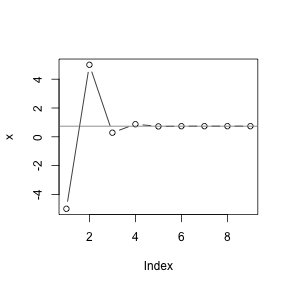
\includegraphics{figures/uniroot-explore1.pdf}

\begin{Shaded}
\begin{Highlighting}[]
\KeywordTok{plot}\NormalTok{(error, }\DataTypeTok{type =} \StringTok{"b"}\NormalTok{); }\KeywordTok{abline}\NormalTok{(}\DataTypeTok{h =} \DecValTok{0}\NormalTok{, }\DataTypeTok{col =} \StringTok{"grey50"}\NormalTok{)}
\end{Highlighting}
\end{Shaded}

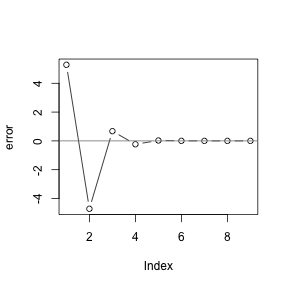
\includegraphics{figures/uniroot-explore2.pdf}

\subsection{Laziness}

The function operators we've seen so far follow a common pattern:

\begin{Shaded}
\begin{Highlighting}[]
\NormalTok{funop <-}\StringTok{ }\NormalTok{function(f, otherargs) \{}
  \NormalTok{function(...) \{}
    \CommentTok{# maybe do something}
    \NormalTok{res <-}\StringTok{ }\KeywordTok{f}\NormalTok{(...)}
    \CommentTok{# maybe do something else}
    \NormalTok{res}
  \NormalTok{\}}
\NormalTok{\}}
\end{Highlighting}
\end{Shaded}

Unfortunately there's a problem with this implementation because
function arguments are lazily evaluated: \texttt{f()} may have changed
between applying the FO and evaluating the function. This is a
particular problem if you're using a for loop or \texttt{lapply()} to
apply multiple function operators. In the following example, we take a
list of functions and delay each one. But when we try to evaluate the
mean, we get the sum instead. \index{lazy evaluation}

\begin{Shaded}
\begin{Highlighting}[]
\NormalTok{funs <-}\StringTok{ }\KeywordTok{list}\NormalTok{(}\DataTypeTok{mean =} \NormalTok{mean, }\DataTypeTok{sum =} \NormalTok{sum)}
\NormalTok{funs_m <-}\StringTok{ }\KeywordTok{lapply}\NormalTok{(funs, delay_by, }\DataTypeTok{delay =} \FloatTok{0.1}\NormalTok{)}

\NormalTok{funs_m$}\KeywordTok{mean}\NormalTok{(}\DecValTok{1}\NormalTok{:}\DecValTok{10}\NormalTok{)}
\CommentTok{#> [1] 55}
\end{Highlighting}
\end{Shaded}

We can avoid that problem by explicitly forcing the evaluation of
\texttt{f()}:

\begin{Shaded}
\begin{Highlighting}[]
\NormalTok{delay_by <-}\StringTok{ }\NormalTok{function(delay, f) \{}
  \KeywordTok{force}\NormalTok{(f)}
  \NormalTok{function(...) \{}
    \KeywordTok{Sys.sleep}\NormalTok{(delay)}
    \KeywordTok{f}\NormalTok{(...)}
  \NormalTok{\}}
\NormalTok{\}}

\NormalTok{funs_m <-}\StringTok{ }\KeywordTok{lapply}\NormalTok{(funs, delay_by, }\DataTypeTok{delay =} \FloatTok{0.1}\NormalTok{)}
\NormalTok{funs_m$}\KeywordTok{mean}\NormalTok{(}\DecValTok{1}\NormalTok{:}\DecValTok{10}\NormalTok{)}
\CommentTok{#> [1] 5.5}
\end{Highlighting}
\end{Shaded}

It's good practice to do that whenever you create a new FO.

\subsection{Exercises}

\begin{enumerate}
\def\labelenumi{\arabic{enumi}.}
\item
  Write a FO that logs a time stamp and message to a file every time a
  function is run.
\item
  What does the following function do? What would be a good name for it?

\begin{Shaded}
\begin{Highlighting}[]
\NormalTok{f <-}\StringTok{ }\NormalTok{function(g) \{}
  \KeywordTok{force}\NormalTok{(g)}
  \NormalTok{result <-}\StringTok{ }\OtherTok{NULL}
  \NormalTok{function(...) \{}
    \NormalTok{if (}\KeywordTok{is.null}\NormalTok{(result)) \{}
      \NormalTok{result <<-}\StringTok{ }\KeywordTok{g}\NormalTok{(...)}
    \NormalTok{\}}
    \NormalTok{result}
  \NormalTok{\}}
\NormalTok{\}}
\NormalTok{runif2 <-}\StringTok{ }\KeywordTok{f}\NormalTok{(runif)}
\KeywordTok{runif2}\NormalTok{(}\DecValTok{5}\NormalTok{)}
\CommentTok{#> [1] 0.37475 0.46234 0.08666 0.94401 0.74132}
\KeywordTok{runif2}\NormalTok{(}\DecValTok{10}\NormalTok{)}
\CommentTok{#> [1] 0.37475 0.46234 0.08666 0.94401 0.74132}
\end{Highlighting}
\end{Shaded}
\item
  Modify \texttt{delay\_by()} so that instead of delaying by a fixed
  amount of time, it ensures that a certain amount of time has elapsed
  since the function was last called. That is, if you called
  \texttt{g \textless{}- delay\_by(1, f); g(); Sys.sleep(2); g()} there
  shouldn't be an extra delay.
\item
  Write \texttt{wait\_until()} which delays execution until a specific
  time.
\item
  There are three places we could have added a memoise call: why did we
  choose the one we did?

\begin{Shaded}
\begin{Highlighting}[]
\NormalTok{download <-}\StringTok{ }\KeywordTok{memoise}\NormalTok{(}\KeywordTok{dot_every}\NormalTok{(}\DecValTok{10}\NormalTok{, }\KeywordTok{delay_by}\NormalTok{(}\DecValTok{1}\NormalTok{, download_file)))}
\NormalTok{download <-}\StringTok{ }\KeywordTok{dot_every}\NormalTok{(}\DecValTok{10}\NormalTok{, }\KeywordTok{memoise}\NormalTok{(}\KeywordTok{delay_by}\NormalTok{(}\DecValTok{1}\NormalTok{, download_file)))}
\NormalTok{download <-}\StringTok{ }\KeywordTok{dot_every}\NormalTok{(}\DecValTok{10}\NormalTok{, }\KeywordTok{delay_by}\NormalTok{(}\DecValTok{1}\NormalTok{, }\KeywordTok{memoise}\NormalTok{(download_file)))}
\end{Highlighting}
\end{Shaded}
\item
  Why is the \texttt{remember()} function inefficient? How could you
  implement it in more efficient way?
\item
  Why does the following code, from
  \href{http://stackoverflow.com/questions/8440675}{stackoverflow}, not
  do what you expect?

\begin{Shaded}
\begin{Highlighting}[]
\CommentTok{# return a linear function with slope a and intercept b.}
\NormalTok{f <-}\StringTok{ }\NormalTok{function(a, b) function(x) a *}\StringTok{ }\NormalTok{x +}\StringTok{ }\NormalTok{b}

\CommentTok{# create a list of functions with different parameters.}
\NormalTok{fs <-}\StringTok{ }\KeywordTok{Map}\NormalTok{(f, }\DataTypeTok{a =} \KeywordTok{c}\NormalTok{(}\DecValTok{0}\NormalTok{, }\DecValTok{1}\NormalTok{), }\DataTypeTok{b =} \KeywordTok{c}\NormalTok{(}\DecValTok{0}\NormalTok{, }\DecValTok{1}\NormalTok{))}

\NormalTok{fs[[}\DecValTok{1}\NormalTok{]](}\DecValTok{3}\NormalTok{)}
\CommentTok{#> [1] 4}
\CommentTok{# should return 0 * 3 + 0 = 0}
\end{Highlighting}
\end{Shaded}

  How can you modify \texttt{f} so that it works correctly?
\end{enumerate}

\hyperdef{}{output-fos}{\section{Output FOs}\label{output-fos}}

The next step up in complexity is to modify the output of a function.
This could be quite simple, or it could fundamentally change the
operation of the function by returning something completely different to
its usual output. In this section you'll learn about two simple
modifications, \texttt{Negate()} and \texttt{failwith()}, and two
fundamental modifications, \texttt{capture\_it()} and
\texttt{time\_it()}.

\subsection{Minor modifications}

\texttt{base::Negate()} and \texttt{plyr::failwith()} offer two minor,
but useful, modifications of a function that are particularly handy in
conjunction with functionals. \indexc{Negate()} \indexc{failwith()}

\texttt{Negate()} takes a function that returns a logical vector (a
predicate function), and returns the negation of that function. This can
be a useful shortcut when a function returns the opposite of what you
need. The essence of \texttt{Negate()} is very simple:

\begin{Shaded}
\begin{Highlighting}[]
\NormalTok{Negate <-}\StringTok{ }\NormalTok{function(f) \{}
  \KeywordTok{force}\NormalTok{(f)}
  \NormalTok{function(...) !}\KeywordTok{f}\NormalTok{(...)}
\NormalTok{\}}
\NormalTok{(}\KeywordTok{Negate}\NormalTok{(is.null))(}\OtherTok{NULL}\NormalTok{)}
\CommentTok{#> [1] FALSE}
\end{Highlighting}
\end{Shaded}

I often use this idea to make a function, \texttt{compact()}, that
removes all null elements from a list: \indexc{compact()}

\begin{Shaded}
\begin{Highlighting}[]
\NormalTok{compact <-}\StringTok{ }\NormalTok{function(x) }\KeywordTok{Filter}\NormalTok{(}\KeywordTok{Negate}\NormalTok{(is.null), x)}
\end{Highlighting}
\end{Shaded}

\texttt{plyr::failwith()} turns a function that throws an error into a
function that returns a default value when there's an error. Again, the
essence of \texttt{failwith()} is simple; it's just a wrapper around
\texttt{try()}, the function that captures errors and allows execution
to continue. \indexc{try()}

\begin{Shaded}
\begin{Highlighting}[]
\NormalTok{failwith <-}\StringTok{ }\NormalTok{function(}\DataTypeTok{default =} \OtherTok{NULL}\NormalTok{, f, }\DataTypeTok{quiet =} \OtherTok{FALSE}\NormalTok{) \{}
  \KeywordTok{force}\NormalTok{(f)}
  \NormalTok{function(...) \{}
    \NormalTok{out <-}\StringTok{ }\NormalTok{default}
    \KeywordTok{try}\NormalTok{(out <-}\StringTok{ }\KeywordTok{f}\NormalTok{(...), }\DataTypeTok{silent =} \NormalTok{quiet)}
    \NormalTok{out}
  \NormalTok{\}}
\NormalTok{\}}
\KeywordTok{log}\NormalTok{(}\StringTok{"a"}\NormalTok{)}
\CommentTok{#> Error: non-numeric argument to mathematical function}
\KeywordTok{failwith}\NormalTok{(}\OtherTok{NA}\NormalTok{, log)(}\StringTok{"a"}\NormalTok{)}
\CommentTok{#> [1] NA}
\KeywordTok{failwith}\NormalTok{(}\OtherTok{NA}\NormalTok{, log, }\DataTypeTok{quiet =} \OtherTok{TRUE}\NormalTok{)(}\StringTok{"a"}\NormalTok{)}
\CommentTok{#> [1] NA}
\end{Highlighting}
\end{Shaded}

(If you haven't seen \texttt{try()} before, it's discussed in more
detail in \hyperref[try]{exceptions and debugging}.)

\texttt{failwith()} is very useful in conjunction with functionals:
instead of the failure propagating and terminating the higher-level
loop, you can complete the iteration and then find out what went wrong.
For example, imagine you're fitting a set of generalised linear models
(GLMs) to a list of data frames. While GLMs can sometimes fail because
of optimisation problems, you'd still want to be able to try to fit all
the models, and later look back at those that failed:
\index{fitting many models}

\begin{Shaded}
\begin{Highlighting}[]
\CommentTok{# If any model fails, all models fail to fit:}
\NormalTok{models <-}\StringTok{ }\KeywordTok{lapply}\NormalTok{(datasets, glm, }\DataTypeTok{formula =} \NormalTok{y ~}\StringTok{ }\NormalTok{x1 +}\StringTok{ }\NormalTok{x2 *}\StringTok{ }\NormalTok{x3)}
\CommentTok{# If a model fails, it will get a NULL value}
\NormalTok{models <-}\StringTok{ }\KeywordTok{lapply}\NormalTok{(datasets, }\KeywordTok{failwith}\NormalTok{(}\OtherTok{NULL}\NormalTok{, glm),}
  \DataTypeTok{formula =} \NormalTok{y ~}\StringTok{ }\NormalTok{x1 +}\StringTok{ }\NormalTok{x2 *}\StringTok{ }\NormalTok{x3)}

\CommentTok{# remove failed models (NULLs) with compact}
\NormalTok{ok_models <-}\StringTok{ }\KeywordTok{compact}\NormalTok{(models)}
\CommentTok{# extract the datasets corresponding to failed models}
\NormalTok{failed_data <-}\StringTok{ }\NormalTok{datasets[}\KeywordTok{vapply}\NormalTok{(models, is.null, }\KeywordTok{logical}\NormalTok{(}\DecValTok{1}\NormalTok{))]}
\end{Highlighting}
\end{Shaded}

I think this is a great example of the power of combining functionals
and function operators: it lets you succinctly express what you need to
solve a common data analysis problem.

\subsection{Changing what a function does}

Other output function operators can have a more profound effect on the
operation of the function. Instead of returning the original return
value, we can return some other effect of the function evaluation. Here
are two examples:

\begin{itemize}
\item
  Return text that the function \texttt{print()}ed:
  \indexc{capture\_it()}

\begin{Shaded}
\begin{Highlighting}[]
\NormalTok{capture_it <-}\StringTok{ }\NormalTok{function(f) \{}
  \KeywordTok{force}\NormalTok{(f)}
  \NormalTok{function(...) \{}
    \KeywordTok{capture.output}\NormalTok{(}\KeywordTok{f}\NormalTok{(...))}
  \NormalTok{\}}
\NormalTok{\}}
\NormalTok{str_out <-}\StringTok{ }\KeywordTok{capture_it}\NormalTok{(str)}
\KeywordTok{str}\NormalTok{(}\DecValTok{1}\NormalTok{:}\DecValTok{10}\NormalTok{)}
\CommentTok{#>  int [1:10] 1 2 3 4 5 6 7 8 9 10}
\KeywordTok{str_out}\NormalTok{(}\DecValTok{1}\NormalTok{:}\DecValTok{10}\NormalTok{)}
\CommentTok{#> [1] " int [1:10] 1 2 3 4 5 6 7 8 9 10"}
\end{Highlighting}
\end{Shaded}
\item
  Return how long a function took to run: \indexc{time\_it()}

\begin{Shaded}
\begin{Highlighting}[]
\NormalTok{time_it <-}\StringTok{ }\NormalTok{function(f) \{}
  \KeywordTok{force}\NormalTok{(f)}
  \NormalTok{function(...) \{}
    \KeywordTok{system.time}\NormalTok{(}\KeywordTok{f}\NormalTok{(...))}
  \NormalTok{\}}
\NormalTok{\}}
\end{Highlighting}
\end{Shaded}
\end{itemize}

\texttt{time\_it()} allows us to rewrite some of the code from the
functionals chapter:

\begin{Shaded}
\begin{Highlighting}[]
\NormalTok{compute_mean <-}\StringTok{ }\KeywordTok{list}\NormalTok{(}
  \DataTypeTok{base =} \NormalTok{function(x) }\KeywordTok{mean}\NormalTok{(x),}
  \DataTypeTok{sum =} \NormalTok{function(x) }\KeywordTok{sum}\NormalTok{(x) /}\StringTok{ }\KeywordTok{length}\NormalTok{(x)}
\NormalTok{)}
\NormalTok{x <-}\StringTok{ }\KeywordTok{runif}\NormalTok{(}\FloatTok{1e6}\NormalTok{)}

\CommentTok{# Previously we used an anonymous function to time execution:}
\CommentTok{# lapply(compute_mean, function(f) system.time(f(x)))}

\CommentTok{# Now we can compose function operators:}
\NormalTok{call_fun <-}\StringTok{ }\NormalTok{function(f, ...) }\KeywordTok{f}\NormalTok{(...)}
\KeywordTok{lapply}\NormalTok{(compute_mean, }\KeywordTok{time_it}\NormalTok{(call_fun), x)}
\CommentTok{#> $base}
\CommentTok{#>    user  system elapsed }
\CommentTok{#>   0.002   0.000   0.002 }
\CommentTok{#> }
\CommentTok{#> $sum}
\CommentTok{#>    user  system elapsed }
\CommentTok{#>   0.001   0.000   0.001}
\end{Highlighting}
\end{Shaded}

In this example, there's not a huge benefit to using function operators,
because the composition is simple and we're applying the same operator
to each function. Generally, using function operators is most effective
when you are using multiple operators or if the gap between creating
them and using them is large.

\subsection{Exercises}

\begin{enumerate}
\def\labelenumi{\arabic{enumi}.}
\item
  Create a \texttt{negative()} FO that flips the sign of the output of
  the function to which it is applied.
\item
  The \texttt{evaluate} package makes it easy to capture all the outputs
  (results, text, messages, warnings, errors, and plots) from an
  expression. Create a function like \texttt{capture\_it()} that also
  captures the warnings and errors generated by a function.
\item
  Create a FO that tracks files created or deleted in the working
  directory (Hint: use \texttt{dir()} and \texttt{setdiff()}.) What
  other global effects of functions might you want to track?
\end{enumerate}

\hyperdef{}{input-fos}{\section{Input FOs}\label{input-fos}}

The next step up in complexity is to modify the inputs of a function.
Again, you can modify how a function works in a minor way (e.g., setting
default argument values), or in a major way (e.g., converting inputs
from scalars to vectors, or vectors to matrices).

\subsection{Prefilling function arguments: partial function application}

A common use of anonymous functions is to make a variant of a function
that has certain arguments ``filled in'' already. This is called
``partial function application'', and is implemented by
\texttt{pryr::partial()}. Once you have read
\hyperref[metaprogramming]{metaprogramming}, I encourage you to read the
source code for \texttt{partial()} and figure out how it works --- it's
only 5 lines of code! \index{partial application} \index{currying}
\indexc{partial()}

\texttt{partial()} allows us to replace code like

\begin{Shaded}
\begin{Highlighting}[]
\NormalTok{f <-}\StringTok{ }\NormalTok{function(a) }\KeywordTok{g}\NormalTok{(a, }\DataTypeTok{b =} \DecValTok{1}\NormalTok{)}
\NormalTok{compact <-}\StringTok{ }\NormalTok{function(x) }\KeywordTok{Filter}\NormalTok{(}\KeywordTok{Negate}\NormalTok{(is.null), x)}
\KeywordTok{Map}\NormalTok{(function(x, y) }\KeywordTok{f}\NormalTok{(x, y, zs), xs, ys)}
\end{Highlighting}
\end{Shaded}

with

\begin{Shaded}
\begin{Highlighting}[]
\NormalTok{f <-}\StringTok{ }\KeywordTok{partial}\NormalTok{(g, }\DataTypeTok{b =} \DecValTok{1}\NormalTok{)}
\NormalTok{compact <-}\StringTok{ }\KeywordTok{partial}\NormalTok{(Filter, }\KeywordTok{Negate}\NormalTok{(is.null))}
\KeywordTok{Map}\NormalTok{(}\KeywordTok{partial}\NormalTok{(f, }\DataTypeTok{zs =} \NormalTok{zs), xs, ys)}
\end{Highlighting}
\end{Shaded}

We can use this idea to simplify the code used when working with lists
of functions. Instead of:

\begin{Shaded}
\begin{Highlighting}[]
\NormalTok{funs2 <-}\StringTok{ }\KeywordTok{list}\NormalTok{(}
  \DataTypeTok{sum =} \NormalTok{function(...) }\KeywordTok{sum}\NormalTok{(..., }\DataTypeTok{na.rm =} \OtherTok{TRUE}\NormalTok{),}
  \DataTypeTok{mean =} \NormalTok{function(...) }\KeywordTok{mean}\NormalTok{(..., }\DataTypeTok{na.rm =} \OtherTok{TRUE}\NormalTok{),}
  \DataTypeTok{median =} \NormalTok{function(...) }\KeywordTok{median}\NormalTok{(..., }\DataTypeTok{na.rm =} \OtherTok{TRUE}\NormalTok{)}
\NormalTok{)}
\end{Highlighting}
\end{Shaded}

we can write:

\begin{Shaded}
\begin{Highlighting}[]
\KeywordTok{library}\NormalTok{(pryr)}
\NormalTok{funs2 <-}\StringTok{ }\KeywordTok{list}\NormalTok{(}
  \DataTypeTok{sum =} \KeywordTok{partial}\NormalTok{(sum, }\DataTypeTok{na.rm =} \OtherTok{TRUE}\NormalTok{),}
  \DataTypeTok{mean =} \KeywordTok{partial}\NormalTok{(mean, }\DataTypeTok{na.rm =} \OtherTok{TRUE}\NormalTok{),}
  \DataTypeTok{median =} \KeywordTok{partial}\NormalTok{(median, }\DataTypeTok{na.rm =} \OtherTok{TRUE}\NormalTok{)}
\NormalTok{)}
\end{Highlighting}
\end{Shaded}

Using partial function application is a straightforward task in many
functional programming languages, but it's not entirely clear how it
should interact with R's lazy evaluation rules. The approach
\texttt{plyr::partial()} takes is to create a function that is as
similar as possible to the anonymous function that you'd create by hand.
Peter Meilstrup takes a different approach in his
\href{https://github.com/crowding/ptools/}{ptools package}. If you're
interested in the topic, you might want to read about the binary
operators he created: \texttt{\%()\%},
\texttt{\%\textgreater{}\textgreater{}\%}, and
\texttt{\%\textless{}\textless{}\%}.

\subsection{Changing input types}

It's also possible to make a major change to a function's input, making
a function work with fundamentally different types of data. There are a
few existing functions that work along these lines:

\begin{itemize}
\item
  \texttt{base::Vectorize()} converts a scalar function to a vector
  function. It takes a non-vectorised function and vectorises it with
  respect to the arguments specified in the \texttt{vectorize.args}
  argument. This doesn't give you any magical performance improvements,
  but it's useful if you want a quick and dirty way of making a
  vectorised function. \indexc{Vectorize()}

  A mildly useful extension to \texttt{sample()} would be to vectorize
  it with respect to size. Doing so would allow you to generate multiple
  samples in one call. \indexc{sample()}

\begin{Shaded}
\begin{Highlighting}[]
\NormalTok{sample2 <-}\StringTok{ }\KeywordTok{Vectorize}\NormalTok{(sample, }\StringTok{"size"}\NormalTok{, }\DataTypeTok{SIMPLIFY =} \OtherTok{FALSE}\NormalTok{)}
\KeywordTok{str}\NormalTok{(}\KeywordTok{sample2}\NormalTok{(}\DecValTok{1}\NormalTok{:}\DecValTok{5}\NormalTok{, }\KeywordTok{c}\NormalTok{(}\DecValTok{1}\NormalTok{, }\DecValTok{1}\NormalTok{, }\DecValTok{3}\NormalTok{)))}
\CommentTok{#> List of 3}
\CommentTok{#>  $ : int 1}
\CommentTok{#>  $ : int 5}
\CommentTok{#>  $ : int [1:3] 1 3 5}
\KeywordTok{str}\NormalTok{(}\KeywordTok{sample2}\NormalTok{(}\DecValTok{1}\NormalTok{:}\DecValTok{5}\NormalTok{, }\DecValTok{5}\NormalTok{:}\DecValTok{3}\NormalTok{))}
\CommentTok{#> List of 3}
\CommentTok{#>  $ : int [1:5] 5 4 1 2 3}
\CommentTok{#>  $ : int [1:4] 4 1 2 5}
\CommentTok{#>  $ : int [1:3] 5 3 2}
\end{Highlighting}
\end{Shaded}

  In this example we have used \texttt{SIMPLIFY = FALSE} to ensure that
  our newly vectorised function always returns a list. This is usually
  what you want.
\item
  \texttt{splat()} converts a function that takes multiple arguments to
  a function that takes a single list of arguments. \indexc{splat()}
  \indexc{do.call()}

\begin{Shaded}
\begin{Highlighting}[]
\NormalTok{splat <-}\StringTok{ }\NormalTok{function (f) \{}
  \KeywordTok{force}\NormalTok{(f)}
  \NormalTok{function(args) \{}
    \KeywordTok{do.call}\NormalTok{(f, args)}
  \NormalTok{\}}
\NormalTok{\}}
\end{Highlighting}
\end{Shaded}

  This is useful if you want to invoke a function with varying
  arguments:

\begin{Shaded}
\begin{Highlighting}[]
\NormalTok{x <-}\StringTok{ }\KeywordTok{c}\NormalTok{(}\OtherTok{NA}\NormalTok{, }\KeywordTok{runif}\NormalTok{(}\DecValTok{100}\NormalTok{), }\DecValTok{1000}\NormalTok{)}
\NormalTok{args <-}\StringTok{ }\KeywordTok{list}\NormalTok{(}
  \KeywordTok{list}\NormalTok{(x),}
  \KeywordTok{list}\NormalTok{(x, }\DataTypeTok{na.rm =} \OtherTok{TRUE}\NormalTok{),}
  \KeywordTok{list}\NormalTok{(x, }\DataTypeTok{na.rm =} \OtherTok{TRUE}\NormalTok{, }\DataTypeTok{trim =} \FloatTok{0.1}\NormalTok{)}
\NormalTok{)}
\KeywordTok{lapply}\NormalTok{(args, }\KeywordTok{splat}\NormalTok{(mean))}
\CommentTok{#> [[1]]}
\CommentTok{#> [1] NA}
\CommentTok{#> }
\CommentTok{#> [[2]]}
\CommentTok{#> [1] 10.41}
\CommentTok{#> }
\CommentTok{#> [[3]]}
\CommentTok{#> [1] 0.5206}
\end{Highlighting}
\end{Shaded}
\item
  \texttt{plyr::colwise()} converts a vector function to one that works
  with data frames: \indexc{colwise()}

\begin{Shaded}
\begin{Highlighting}[]
\KeywordTok{median}\NormalTok{(mtcars)}
\CommentTok{#> Error: need numeric data}
\KeywordTok{median}\NormalTok{(mtcars$mpg)}
\CommentTok{#> [1] 19.2}
\NormalTok{plyr::}\KeywordTok{colwise}\NormalTok{(median)(mtcars)}
\CommentTok{#>    mpg cyl  disp  hp  drat    wt  qsec vs am gear carb}
\CommentTok{#> 1 19.2   6 196.3 123 3.695 3.325 17.71  0  0    4    2}
\end{Highlighting}
\end{Shaded}
\end{itemize}

\subsection{Exercises}

\begin{enumerate}
\def\labelenumi{\arabic{enumi}.}
\item
  Our previous \texttt{download()} function only downloads a single
  file. How can you use \texttt{partial()} and \texttt{lapply()} to
  create a function that downloads multiple files at once? What are the
  pros and cons of using \texttt{partial()} vs. writing a function by
  hand?
\item
  Read the source code for \texttt{plyr::colwise()}. How does the code
  work? What are \texttt{colwise()}'s three main tasks? How could you
  make \texttt{colwise()} simpler by implementing each task as a
  function operator? (Hint: think about \texttt{partial()}.)
\item
  Write FOs that convert a function to return a matrix instead of a data
  frame, or a data frame instead of a matrix. If you understand S3, call
  them \texttt{as.data.frame.function()} and
  \texttt{as.matrix.function()}.
\item
  You've seen five functions that modify a function to change its output
  from one form to another. What are they? Draw a table of the various
  combinations of types of outputs: what should go in the rows and what
  should go in the columns? What function operators might you want to
  write to fill in the missing cells? Come up with example use cases.
\item
  Look at all the examples of using an anonymous function to partially
  apply a function in this and the previous chapter. Replace the
  anonymous function with \texttt{partial()}. What do you think of the
  result? Is it easier or harder to read?
\end{enumerate}

\hyperdef{}{combining-fos}{\section{Combining FOs}\label{combining-fos}}

Besides just operating on single functions, function operators can take
multiple functions as input. One simple example of this is
\texttt{plyr::each()}. It takes a list of vectorised functions and
combines them into a single function. \indexc{each()}

\begin{Shaded}
\begin{Highlighting}[]
\NormalTok{summaries <-}\StringTok{ }\NormalTok{plyr::}\KeywordTok{each}\NormalTok{(mean, sd, median)}
\KeywordTok{summaries}\NormalTok{(}\DecValTok{1}\NormalTok{:}\DecValTok{10}\NormalTok{)}
\CommentTok{#>   mean     sd median }
\CommentTok{#>  5.500  3.028  5.500}
\end{Highlighting}
\end{Shaded}

Two more complicated examples are combining functions through
composition, or through boolean algebra. These capabilities are the glue
that allow us to join multiple functions together.

\subsection{Function composition}

An important way of combining functions is through composition:
\texttt{f(g(x))}. Composition takes a list of functions and applies them
sequentially to the input. It's a replacement for the common pattern of
anonymous function that chains multiple functions together to get the
result you want: \index{functions!composition of} \index{composition}
\indexc{compose()}

\begin{Shaded}
\begin{Highlighting}[]
\KeywordTok{sapply}\NormalTok{(mtcars, function(x) }\KeywordTok{length}\NormalTok{(}\KeywordTok{unique}\NormalTok{(x)))}
\CommentTok{#>  mpg  cyl disp   hp drat   wt qsec   vs   am gear carb }
\CommentTok{#>   25    3   27   22   22   29   30    2    2    3    6}
\end{Highlighting}
\end{Shaded}

A simple version of compose looks like this:

\begin{Shaded}
\begin{Highlighting}[]
\NormalTok{compose <-}\StringTok{ }\NormalTok{function(f, g) \{}
  \NormalTok{function(...) }\KeywordTok{f}\NormalTok{(}\KeywordTok{g}\NormalTok{(...))}
\NormalTok{\}}
\end{Highlighting}
\end{Shaded}

(\texttt{pryr::compose()} provides a more full-featured alternative that
can accept multiple functions and is used for the rest of the examples.)

This allows us to write:

\begin{Shaded}
\begin{Highlighting}[]
\KeywordTok{sapply}\NormalTok{(mtcars, }\KeywordTok{compose}\NormalTok{(length, unique))}
\CommentTok{#>  mpg  cyl disp   hp drat   wt qsec   vs   am gear carb }
\CommentTok{#>   25    3   27   22   22   29   30    2    2    3    6}
\end{Highlighting}
\end{Shaded}

Mathematically, function composition is often denoted with the infix
operator, o, \texttt{(f o g)(x)}. Haskell, a popular functional
programming language, uses \texttt{.} to the same end. In R, we can
create our own infix composition function: \indexc{\%o\%}

\begin{Shaded}
\begin{Highlighting}[]
\StringTok{"%o%"} \NormalTok{<-}\StringTok{ }\NormalTok{compose}
\KeywordTok{sapply}\NormalTok{(mtcars, length %o%}\StringTok{ }\NormalTok{unique)}
\CommentTok{#>  mpg  cyl disp   hp drat   wt qsec   vs   am gear carb }
\CommentTok{#>   25    3   27   22   22   29   30    2    2    3    6}

\KeywordTok{sqrt}\NormalTok{(}\DecValTok{1} \NormalTok{+}\StringTok{ }\DecValTok{8}\NormalTok{)}
\CommentTok{#> [1] 3}
\KeywordTok{compose}\NormalTok{(sqrt, }\StringTok{`}\DataTypeTok{+}\StringTok{`}\NormalTok{)(}\DecValTok{1}\NormalTok{, }\DecValTok{8}\NormalTok{)}
\CommentTok{#> [1] 3}
\NormalTok{(sqrt %o%}\StringTok{ `}\DataTypeTok{+}\StringTok{`}\NormalTok{)(}\DecValTok{1}\NormalTok{, }\DecValTok{8}\NormalTok{)}
\CommentTok{#> [1] 3}
\end{Highlighting}
\end{Shaded}

Compose also allows for a very succinct implementation of
\texttt{Negate}, which is just a partially evaluated version of
\texttt{compose()}. \indexc{Negate()}

\begin{Shaded}
\begin{Highlighting}[]
\NormalTok{Negate <-}\StringTok{ }\KeywordTok{partial}\NormalTok{(compose, }\StringTok{`}\DataTypeTok{!}\StringTok{`}\NormalTok{)}
\end{Highlighting}
\end{Shaded}

We could implement the population standard deviation with function
composition:

\begin{Shaded}
\begin{Highlighting}[]
\NormalTok{square <-}\StringTok{ }\NormalTok{function(x) x^}\DecValTok{2}
\NormalTok{deviation <-}\StringTok{ }\NormalTok{function(x) x -}\StringTok{ }\KeywordTok{mean}\NormalTok{(x)}

\NormalTok{sd2 <-}\StringTok{ }\NormalTok{sqrt %o%}\StringTok{ }\NormalTok{mean %o%}\StringTok{ }\NormalTok{square %o%}\StringTok{ }\NormalTok{deviation}
\KeywordTok{sd2}\NormalTok{(}\DecValTok{1}\NormalTok{:}\DecValTok{10}\NormalTok{)}
\CommentTok{#> [1] 2.872}
\end{Highlighting}
\end{Shaded}

This type of programming is called tacit or point-free programming. (The
term point-free comes from the use of ``point'' to refer to values in
topology; this style is also derogatorily known as pointless). In this
style of programming, you don't explicitly refer to variables. Instead,
you focus on the high-level composition of functions rather than the
low-level flow of data. The focus is on what's being done, not on
objects it's being done to. Since we're using only functions and not
parameters, we use verbs and not nouns. This style is common in Haskell,
and is the typical style in stack based programming languages like Forth
and Factor. It's not a terribly natural or elegant style in R, but it is
fun to play with. \index{point-free programming}
\index{tacit programming}

\texttt{compose()} is particularly useful in conjunction with
\texttt{partial()}, because \texttt{partial()} allows you to supply
additional arguments to the functions being composed. One nice side
effect of this style of programming is that it keeps a function's
arguments near its name. This is important because as the size of the
chunk of code you have to hold in your head grows code becomes harder to
understand.

Below I take the example from the first section of the chapter and
modify it to use the two styles of function composition described above.
Both results are longer than the original code, but they may be easier
to understand because the function and its arguments are closer
together. Note that we still have to read them from right to left
(bottom to top): the first function called is the last one written. We
could define \texttt{compose()} to work in the opposite direction, but
in the long run, this is likely to lead to confusion since we'd create a
small part of the langugage that reads differently from every other
part.

\begin{Shaded}
\begin{Highlighting}[]
\NormalTok{download <-}\StringTok{ }\KeywordTok{dot_every}\NormalTok{(}\DecValTok{10}\NormalTok{, }\KeywordTok{memoise}\NormalTok{(}\KeywordTok{delay_by}\NormalTok{(}\DecValTok{1}\NormalTok{, download_file)))}

\NormalTok{download <-}\StringTok{ }\NormalTok{pryr::}\KeywordTok{compose}\NormalTok{(}
  \KeywordTok{partial}\NormalTok{(dot_every, }\DecValTok{10}\NormalTok{),}
  \NormalTok{memoise,}
  \KeywordTok{partial}\NormalTok{(delay_by, }\DecValTok{1}\NormalTok{),}
  \NormalTok{download_file}
\NormalTok{)}

\NormalTok{download <-}\StringTok{ }\KeywordTok{partial}\NormalTok{(dot_every, }\DecValTok{10}\NormalTok{) %o%}
\StringTok{  }\NormalTok{memoise %o%}
\StringTok{  }\KeywordTok{partial}\NormalTok{(delay_by, }\DecValTok{1}\NormalTok{) %o%}
\StringTok{  }\NormalTok{download_file}
\end{Highlighting}
\end{Shaded}

\subsection{Logical predicates and boolean algebra}

When I use \texttt{Filter()} and other functionals that work with
logical predicates, I often find myself using anonymous functions to
combine multiple conditions: \index{predicate functions}

\begin{Shaded}
\begin{Highlighting}[]
\KeywordTok{Filter}\NormalTok{(function(x) }\KeywordTok{is.character}\NormalTok{(x) ||}\StringTok{ }\KeywordTok{is.factor}\NormalTok{(x), iris)}
\end{Highlighting}
\end{Shaded}

As an alternative, we could define function operators that combine
logical predicates:

\begin{Shaded}
\begin{Highlighting}[]
\NormalTok{and <-}\StringTok{ }\NormalTok{function(f1, f2) \{}
  \KeywordTok{force}\NormalTok{(f1); }\KeywordTok{force}\NormalTok{(f2)}
  \NormalTok{function(...) \{}
    \KeywordTok{f1}\NormalTok{(...) &&}\StringTok{ }\KeywordTok{f2}\NormalTok{(...)}
  \NormalTok{\}}
\NormalTok{\}}
\NormalTok{or <-}\StringTok{ }\NormalTok{function(f1, f2) \{}
  \KeywordTok{force}\NormalTok{(f1); }\KeywordTok{force}\NormalTok{(f2)}
  \NormalTok{function(...) \{}
    \KeywordTok{f1}\NormalTok{(...) ||}\StringTok{ }\KeywordTok{f2}\NormalTok{(...)}
  \NormalTok{\}}
\NormalTok{\}}
\NormalTok{not <-}\StringTok{ }\NormalTok{function(f1) \{}
  \KeywordTok{force}\NormalTok{(f1); }\KeywordTok{force}\NormalTok{(f2)}
  \NormalTok{function(...) \{}
    \NormalTok{!}\KeywordTok{f1}\NormalTok{(...)}
  \NormalTok{\}}
\NormalTok{\}}
\end{Highlighting}
\end{Shaded}

This would allow us to write:

\begin{Shaded}
\begin{Highlighting}[]
\KeywordTok{Filter}\NormalTok{(}\KeywordTok{or}\NormalTok{(is.character, is.factor), iris)}
\end{Highlighting}
\end{Shaded}

And we now have a boolean algebra on functions, not on the results of
functions. \index{Boolean algebra}

\subsection{Exercises}

\begin{enumerate}
\def\labelenumi{\arabic{enumi}.}
\item
  Implement your own version of \texttt{compose()} using \texttt{Reduce}
  and \texttt{\%o\%}. For bonus points, do it without calling
  \texttt{function}.
\item
  Extend \texttt{and()} and \texttt{or()} to deal with any number of
  input functions. Can you do it with \texttt{Reduce()}? Can you keep
  them lazy (e.g., for \texttt{and()}, the function returns once it sees
  the first \texttt{FALSE})?
\item
  Implement the \texttt{xor()} binary operator. Implement it using the
  existing \texttt{xor()} function. Implement it as a combination of
  \texttt{and()} and \texttt{or()}. What are the advantages and
  disadvantages of each approach? Also think about what you'll call the
  resulting function to avoid a clash with the existing \texttt{xor()}
  function, and how you might change the names of \texttt{and()},
  \texttt{not()}, and \texttt{or()} to keep them consistent.
\item
  Above, we implemented boolean algebra for functions that return a
  logical function. Implement elementary algebra (\texttt{plus()},
  \texttt{minus()}, \texttt{multiply()}, \texttt{divide()},
  \texttt{exponentiate()}, \texttt{log()}) for functions that return
  numeric vectors.
\end{enumerate}
